% The following text is common to slides.tex, slides_notes.tex and slides_handout.tex

\usepackage[utf8]{inputenc}
\usepackage[T1]{fontenc}

% English environment
%\usepackage[english]{babel}

% French environment
\usepackage[french]{babel}

% French + English environment
%\usepackage[francais,english]{babel}

%%%%%%%%%%%%%%%%%%%%%%%%%%%%%%%%%%%%%%%%%%%%%%%%%%%%%%%%%%%%%%%%%%%%%%%%%%%%%%%%

\usepackage{algorithm}
\usepackage{algorithmic}
\usepackage{amsmath}
\usepackage{amssymb}
%\usepackage{bm}    % bold math
\usepackage{color} % change text color
\usepackage{epsfig}
\usepackage{eurosym}
\usepackage{graphicx}
\usepackage{ifthen}
%\usepackage{natbib} % For bibliography, often used nowadays
\usepackage{rotating}
\usepackage{subfigure}
\usepackage{url}

% TikZ %%%%%%%%%%%%%%%%%%%%%%%%%%%%%%%%%%%%%%%%%%%%%%%%%%%%%%%%%%%%%%%%%%%%%%%%

%\usepackage{tikz}
%\usetikzlibrary{matrix} % for block alignment
\usetikzlibrary{arrows} % for arrow heads
\usetikzlibrary{calc}   % for manipulation of coordinates
\usetikzlibrary{positioning} 
\usetikzlibrary{patterns}



% Listings package settings %%%%%%%%%%%%%%%%%%%%%%%%%%%%%%%%%%%%%%%%%%%%%%%%%%%%

\usepackage{listings}

% Listings package settings %%%%%%%%%%%%%%%%%%%%%%%%%%%%%%%%%%%%%%%%%%%%%%%%%%%%

% See http://en.wikibooks.org/wiki/LaTeX/Source_Code_Listings

% By default, listings does not support multi-byte encoding for source code. The extendedchar option only works for 8-bits encodings such as latin1.
% To handle UTF-8, you should tell listings how to interpret the special characters by defining them like so
\lstset{literate=
    {á}{{\'a}}1 {é}{{\'e}}1 {í}{{\'i}}1 {ó}{{\'o}}1 {ú}{{\'u}}1
    {Á}{{\'A}}1 {É}{{\'E}}1 {Í}{{\'I}}1 {Ó}{{\'O}}1 {Ú}{{\'U}}1
    {à}{{\`a}}1 {è}{{\'e}}1 {ì}{{\`i}}1 {ò}{{\`o}}1 {ù}{{\`u}}1
    {À}{{\`A}}1 {È}{{\'E}}1 {Ì}{{\`I}}1 {Ò}{{\`O}}1 {Ù}{{\`U}}1
    {ä}{{\"a}}1 {ë}{{\"e}}1 {ï}{{\"i}}1 {ö}{{\"o}}1 {ü}{{\"u}}1
    {Ä}{{\"A}}1 {Ë}{{\"E}}1 {Ï}{{\"I}}1 {Ö}{{\"O}}1 {Ü}{{\"U}}1
    {â}{{\^a}}1 {ê}{{\^e}}1 {î}{{\^i}}1 {ô}{{\^o}}1 {û}{{\^u}}1
    {Â}{{\^A}}1 {Ê}{{\^E}}1 {Î}{{\^I}}1 {Ô}{{\^O}}1 {Û}{{\^U}}1
    {œ}{{\oe}}1 {Œ}{{\OE}}1 {æ}{{\ae}}1 {Æ}{{\AE}}1 {ß}{{\ss}}1
    {ç}{{\c c}}1 {Ç}{{\c C}}1 {ø}{{\o}}1 {å}{{\r a}}1 {Å}{{\r A}}1
    {€}{{\EUR}}1 {£}{{\pounds}}1
}

\usepackage{color}

\definecolor{mygreen}{rgb}{0,0.6,0}
\definecolor{mygray}{rgb}{0.5,0.5,0.5}
\definecolor{mymauve}{rgb}{0.58,0,0.82}

\lstset{ %
  backgroundcolor=\color{white},   % choose the background color; you must add \usepackage{color} or \usepackage{xcolor}
  basicstyle=\footnotesize,        % the size of the fonts that are used for the code
  breakatwhitespace=false,         % sets if automatic breaks should only happen at whitespace
  breaklines=true,                 % sets automatic line breaking
  captionpos=b,                    % sets the caption-position to bottom
  commentstyle=\color{mygreen},    % comment style
  deletekeywords={...},            % if you want to delete keywords from the given language
  escapeinside={\%*}{*)},          % if you want to add LaTeX within your code
  extendedchars=true,              % lets you use non-ASCII characters; for 8-bits encodings only, does not work with UTF-8
  frame=L,                    % adds a frame around the code
  keepspaces=true,                 % keeps spaces in text, useful for keeping indentation of code (possibly needs columns=flexible)
  keywordstyle=\color{blue},       % keyword style
  %language=Octave,                % the language of the code
  morekeywords={*,...},            % if you want to add more keywords to the set
  numbers=left,                    % where to put the line-numbers; possible values are (none, left, right)
  numbersep=10pt,                  % how far the line-numbers are from the code
  numberstyle=\tiny\color{mygray}, % the style that is used for the line-numbers
  rulecolor=\color{black},         % if not set, the frame-color may be changed on line-breaks within not-black text (e.g. comments (green here))
  showspaces=false,                % show spaces everywhere adding particular underscores; it overrides 'showstringspaces'
  showstringspaces=false,          % underline spaces within strings only
  showtabs=false,                  % show tabs within strings adding particular underscores
  stepnumber=1,                    % the step between two line-numbers. If it's 1, each line will be numbered
  stringstyle=\color{mymauve},     % string literal style
  tabsize=2,                       % sets default tabsize to 2 spaces
  title=\lstname                   % show the filename of files included with \lstinputlisting; also try caption instead of title
}

\lstdefinestyle{customc}{
  belowcaptionskip=1\baselineskip,
  breaklines=true,
  frame=L,
  xleftmargin=\parindent,
  language=C,
  showstringspaces=false,
  basicstyle=\footnotesize\ttfamily,
  keywordstyle=\bfseries\color{green!40!black},
  commentstyle=\itshape\color{purple!40!black},
  identifierstyle=\color{blue},
  stringstyle=\color{orange},
}

\lstdefinestyle{customasm}{
  belowcaptionskip=1\baselineskip,
  frame=L,
  xleftmargin=\parindent,
  language=[x86masm]Assembler,
  basicstyle=\footnotesize\ttfamily,
  commentstyle=\itshape\color{purple!40!black},
}

\lstset{escapechar=@,style=customc}




%% COMMANDS AND DEFS %%%%%%%%%%%%%%%%%%%%%%%%%%%%%%%%%%%%%%%%%%%%%%%%%%%%%%%%%%%

% Pour désactiver temporairement les images (compile beaucoup plus vite)
%\renewcommand{\includegraphics}[2][]{\null}

%%% Math symbols

%\renewcommand{\vec}[1]{\ensuremath{\boldsymbol{#1}}} % bold vectors
\newcommand{\vs}[1]{\boldsymbol{#1}} % vector symbol (\boldsymbol, \textbf or \vec)
\newcommand{\ms}[1]{\boldsymbol{#1}} % matrix symbol (\boldsymbol, \textbf)

\newcommand{\x}{\vs{x}}
\newcommand{\xstar}{\vs{x^*}}
\newcommand{\w}{\vs{\omega}}
\newcommand{\objfunc}{f}

\def\bbbr{{\rm I\!R}} % reelle Zahlen

\newcommand{\E}{\mathbb{E}}
\newcommand{\N}{\mathbb{N}}
\newcommand{\Z}{\mathbb{Z}}
\newcommand{\Q}{\mathbb{Q}}
\newcommand{\R}{{\bbbr}{}}
\newcommand{\C}{\mathbb{C}}
\newcommand{\K}{\mathbb{K}}

\newcommand{\mb}[1]{\mathbb{#1}}
\newcommand{\mc}[1]{\mathcal{#1}}

\def\CQFD{\fbox\\}

%%% General commands

\newenvironment{jmatrix}{\renewcommand\arraystretch{1.5} \begin{pmatrix}}{\end{pmatrix}}
%\renewcommand{\arraystretch}{1.5}

\newcommand{\cred}[1]{\textcolor{red}{#1}}
\newcommand{\ech}[1]{\textcolor{gray}{#1}}
\newcommand{\imp}[1]{{\em {#1}}}
\newcommand{\voc}[1]{{\em {#1}}}
\newcommand{\todo}[1][\dots]{\textbf{[TODO : #1]}}  % todo mark

\newcommand{\dontforget}[1]{\textcolor{red}{#1}}

\newcommand{\HRule}{\rule{\linewidth}{0.5mm}}

%%% Debug: Display the current table counter (cf. http://www.iam.ubc.ca/old_pages/newbury/tex/numbering.html)

\newcommand{\tablecounterdebug}{\textbf{Table~counter:~\thetable}\\}
\newcommand{\equationcounterdebug}{\textbf{Equation~counter:~\theequation}\\}
\newcommand{\figurecounterdebug}{\textbf{Figure~counter:~\thefigure}\\}
\newcommand{\algorithmcounterdebug}{\textbf{Algorithm~counter:~\thealgorithm}\\}



\usetheme[compress]{Dresden}

%%%%%%%%%%%%%%%%%%%%%%%%%%%%%%%%%%%%%%%%%%%%%%%%%%%%%%%%%%%%%%%%%%%%%%%%%%%%%%%

\title{Put a title here\\on multiple lines if needed}
\subtitle{Put a subtitle here}

% \author[⟨short author names⟩]{⟨author names⟩}
% The names should be separated using the command \and.
\author[Decock]{Jeremie~Decock}

%\institute{Inria}

\date{\today}

% \subject{⟨text⟩}
% Enters the ⟨text⟩ as the subject text in the pdf document info.
% It currently has no other effect.
\subject{The subject of the presentation}

% \keywords{⟨text⟩}
% Enters the ⟨text⟩ as keywords in the pdf document info.
% It currently has no other effect. 
\keywords{put, key, words, here}


%%%%%%%%%%%%%%%%%%%%%%%%%%%%%%%%%%%%%%%%%%%%%%%%%%%%%%%%%%%%%%%%%%%%%%%%%%%%%%%

\begin{document}

\begin{frame}
    \titlepage
\end{frame}
\note{
}

%% Define the logo
%\logo{
\includegraphics[height=0.7cm]{fig/inr_logo_cherch_UK_coul}}

%% Redefini le logo : pour tous les slides suivants
%% logo est remplace par le numero de page
%\setbeamercolor*{logo}{fg=black}
%\logo{\insertframenumber}
%%\logo{\insertframenumber/\inserttotalframenumber}

%%%%%%%%%%%%%%%%%%%%%%%%%%%%%%%%%%%%%%%%%%%%%%%%%%%%%%%%%%%%%%%%%%%%%%%%%%%%%%%

\section*{Introduction}

\begin{frame}{Introduction}
    \dots
\end{frame}
\note{
}



\begin{frame}{Overview}
    \tableofcontents[hideallsubsections]
\end{frame}
\note{
}

\section{Section}

\subsection{Subsection}

\begin{frame}{Title}{Subtitle}
    \begin{itemize}
        \item 
        \item 
        \item 
    \end{itemize}
\end{frame}
\note{
}

\begin{frame}{Title}{Subtitle}
    \begin{itemize}
        \item 
        \item 
        \item 
    \end{itemize}
\end{frame}
\note{
}

\begin{frame}{Title}{Subtitle}
    \begin{itemize}
        \item 
        \item 
        \item 
    \end{itemize}
\end{frame}
\note{
}


\section{Snippets}

\subsection{Snippets}

\begin{frame}{Basic frame}{Subtitle}
    \dots
\end{frame}
\note{
Add some notes\dots
}

\begin{frame}{Citations and references}{cite, label and ref commands}
    Eq. (\ref{eq:bellman}) define the Bellman equation \cite{bellman1956dynamic}
    \begin{equation}
        V(x) = \max_{a \in \Gamma (x) } \{ F(x,a) + \beta V(T(x,a)) \}  \label{eq:bellman}
    \end{equation}
\end{frame}
\note{
}


\begin{frame}{Lists}{itemize, enumerate and description commands}
    \begin{itemize}
        \item item 1
        \item item 2
        \item \dots
    \end{itemize}

    \begin{enumerate}
        \item item 1
        \item item 2
        \item \dots
    \end{enumerate}

    \begin{description}
        \item[First] item 1
        \item[Second] item 2
        \item[Last] \dots
    \end{description}
\end{frame}
\note{
}


\begin{frame}{Colors}{color environment}
    \begin{small}
    small
    \end{small}

    \begin{footnotesize}
    footnotesize
    \end{footnotesize}

    \begin{scriptsize}
    scriptsize
    \end{scriptsize}

    \begin{tiny}
    tiny
    \end{tiny}
\end{frame}
\note{
}


\begin{frame}{Fonts color}{color environment}
    {\color{red} Red}
    {\color{green} Green}
    {\color{blue} Blue}
\end{frame}
\note{
}


\begin{frame}{Centered image}{includegraphics command}
    \begin{center}
        
\includegraphics[width=.80\linewidth]{fig/test}
    \end{center}
\end{frame}
\note{
}

\begin{frame}{Subfigures}{figure, subfigure and includegraphics commands}
    \begin{figure}
        \centering
        \subfigure{
\includegraphics[width=.30\linewidth,height=.20\linewidth]{fig/test}}~
        \subfigure{
\includegraphics[width=.30\linewidth,height=.20\linewidth]{fig/test}}~
        \subfigure{
\includegraphics[width=.30\linewidth,height=.20\linewidth]{fig/test}}
        ~\\
        \subfigure{
\includegraphics[width=.30\linewidth,height=.20\linewidth]{fig/test}}~
        \subfigure{
\includegraphics[width=.30\linewidth,height=.20\linewidth]{fig/test}}~
        \subfigure{
\includegraphics[width=.30\linewidth,height=.20\linewidth]{fig/test}}
    \end{figure}
\end{frame}
\note{
}


\begin{frame}{Blocks}{block command}
    \begin{block}{Block 1}
        Blablabla
    \end{block}

    ~\\

    \begin{block}{Block 2}
        Blablabla
    \end{block}
\end{frame}
\note{
}


\begin{frame}{Equations}
    $$
        V(x) = \max_{a \in \Gamma (x) } \{ F(x,a) + \beta V(T(x,a)) \}  \label{eq:bellman}
    $$

    \[
        V(x) = \max_{a \in \Gamma (x) } \{ F(x,a) + \beta V(T(x,a)) \}  \label{eq:bellman}
    \]

    \begin{equation}
        V(x) = \max_{a \in \Gamma (x) } \{ F(x,a) + \beta V(T(x,a)) \}  \label{eq:bellman}
    \end{equation}
\end{frame}
\note{
}



\begin{frame}{Equation array}{eqnarray command}
    \begin{tiny}
        \begin{eqnarray*}
            \mbox{Expectation of N} & = & \sum_{i=1}^{n} \E(Z_i) \\
                                    & = & \sum_{i=1}^{n} \frac{\gamma}{d^{\beta/2}} \frac{ c(d)^\beta }{i^{\alpha\beta}} \\
                                    & = & \frac{\gamma}{d^{\beta/2}} c(d)^\beta \sum_{i=1}^{n} \frac{1}{i^{\alpha\beta}} \\
                                    & = & z \\
                                    & ~ & \\
        \end{eqnarray*}
        \begin{eqnarray}
            \mbox{Variance of N} & = & \sum_{i=1}^{n} V(Z_i) \\
                                 & \leq & \sum_{i=1}^{n} \E(Z_i) ~~~~~~~ (\mbox{as } V(Z_i) \leq \E(Z_i)) \\
                                 & \leq & z  \nonumber
        \end{eqnarray}
    \end{tiny}
\end{frame}
\note{
}


\begin{frame}{Matrices}
    \begin{small}
        $$
            A_{m,n} =
            \begin{pmatrix}
                a_{1,1} & a_{1,2} & \cdots & a_{1,n} \\
                a_{2,1} & a_{2,2} & \cdots & a_{2,n} \\
                \vdots  & \vdots  & \ddots & \vdots  \\
                a_{m,1} & a_{m,2} & \cdots & a_{m,n}
            \end{pmatrix}
        $$

        $$
            M =
            \begin{bmatrix}
                \frac{5}{6} & \frac{1}{6} & 0           \\[0.3em]
                \frac{5}{6} & 0           & \frac{1}{6} \\[0.3em]
                0           & \frac{5}{6} & \frac{1}{6}
            \end{bmatrix}
        $$

        $$
            M = \bordermatrix{~ & x & y \cr
                              A & 1 & 0 \cr
                              B & 0 & 1 \cr}
        $$
    \end{small}
\end{frame}
\note{
}


\begin{frame}{Systems of equation array}
    \[
        f(n) = \left\{
        \begin{array}{l l}
            n/2      & \quad \text{if $n$ is even}\\
            -(n+1)/2 & \quad \text{if $n$ is odd}
        \end{array} \right.
    \]
\end{frame}
\note{
}


\begin{frame}{Mathematical programming}{with align}
    \begin{align}
        \max        & \quad z = 4 x_1 + 7 x_2    \notag \\
        \text{s.t.} & \quad 3 x_1 + 5 x_2 \leq 6 \label{constraint1}\\
                    & \quad   x_1 + 2 x_2 \leq 8 \label{constraint2}\\
                    & \quad   x_1, x_2 \geq 0    \notag
    \end{align}
\end{frame}
\note{
}


\begin{frame}{Mathematical programming}{with alignat}

    % see http://tex.stackexchange.com/questions/75108/how-to-edit-the-linear-programming-in-latex
    % and http://tex.stackexchange.com/questions/83918/labeled-linear-program-with-labeled-equations-and-wide-objective-function

    % see http://latex.wikia.com/wiki/List_of_LaTeX_environments for explanations about alignat

    % The alignat environment can be used to align equations, and explicitly
    % specify the number of "equation" columns. An equation column has two
    % parts, separated by the equals-sign. Essentially, this is an array with
    % alternating right-aligned and left-aligned columns. The required
    % parameter of alignat is the maximum number of ampersands in a row plus 1,
    % and then divided by 2. One use of alignat is to explicitly specify the
    % amount of horizontal space between columns by including the required
    % spacing in the first row.

    % \rlap is used since the operators in the first equation have no business
    % being aligned with the rest.

    \begin{scriptsize}
        %\begin{alignat*}{6}   % argument = at least (the number of '&' + 1) / 2
        %    \text{Max}  \quad \rlap{$z = x_1 + 12x_2$}                                       \\               
        %    \text{s.t.} \quad & 13 & x_1 & {}+{} &  & x_2 & {}+{} & 12 & x_3 & ~ \leq ~ & 5  \\
        %                      &    & x_1 &       &  &     & {}+{} &    & x_3 & ~ \leq ~ & 16 \\
        %                      & 15 & x_1 & {}+{} &  & x_2 &       &    &     & ~ =    ~ & 14 \\
        %                      & \rlap{$x_j \geqslant 0,\; j=1,2,3.$}
        %\end{alignat*}

        \begin{alignat*}{5}  % argument = at least (the number of '&' + 1) / 2
            \text{Max}  \quad \rlap{$z = x_1 + 12x_2$}                                   \\               
            \text{s.t.} \quad & & 13 x_1 & {}+{} &  x_2 & {}+{} & 12 x_3 & ~ \leq ~ & 5  \\
                              & &    x_1 &       &      & {}+{} &    x_3 & ~ \leq ~ & 16 \\
                              & & 15 x_1 & {}+{} &  x_2 &       &        & ~ =    ~ & 14 \\
                              & \rlap{$x_j \geq 0, ~ j=1,2,3.$}
        \end{alignat*}

        \begin{alignat}{5}   % argument = at least (the number of '&' + 1) / 2
            \text{Max}  \quad \rlap{$z = x_1 + 12x_2$}                                  \nonumber  \\
            \text{s.t.} \quad & & 13 x_1 & {}+{} & x_2 & {}+{} & 12 x_3 & ~ \leq ~ & 5  \label{c1} \\
                              & &    x_1 &       &     & {}+{} &    x_3 & ~ \leq ~ & 16 \label{c2} \\
                              & & 15 x_1 & {}+{} & x_2 &       &        & ~ =    ~ & 14 \label{c3} \\
                              & \rlap{$x_j \geq 0, ~ j=1,2,3.$}                         \nonumber
        \end{alignat}
    \end{scriptsize}

\end{frame}
\note{
}


\begin{frame}{Animations}
    \only<1| handout:0> {
        Slide 1
        \begin{itemize}
            \item \dots
            \item \dots
        \end{itemize}
    }

    \only<2| handout:0> {
        Slide 2
        \begin{itemize}
            \item \dots
            \item \dots
        \end{itemize}
    }

    \only<3| handout:0> {
        Slide 3
        \begin{itemize}
            \item \dots
            \item \dots
        \end{itemize}
    }
\end{frame}
\note{
}

% Algorithmic commands:
%  \STATE <text>
%  \IF{<condition>} \STATE{<text>} \ENDIF
%  \FOR{<condition>} \STATE{<text>} \ENDFOR
%  \FOR{<condition> \TO <condition> } \STATE{<text>} \ENDFOR
%  \FORALL{<condition>} \STATE{<text>} \ENDFOR
%  \WHILE{<condition>} \STATE{<text>} \ENDWHILE
%  \REPEAT \STATE{<text>} \UNTIL{<condition>}
%  \LOOP \STATE{<text>} \ENDLOOP
%  \REQUIRE <text>
%  \ENSURE <text>
%  \RETURN <text>
%  \PRINT <text>
%  \COMMENT{<text>}
%  \AND, \OR, \XOR, \NOT, \TO, \TRUE, \FALSE
\begin{frame}{Algorithms}{algorithmic command}
    \begin{scriptsize}
        \begin{algorithmic}
            \REQUIRE ~\\
                     $\langle \S, \A, T, R \rangle$, an MDP\\
                     $\discount$, the discount factor\\
                     $\epsilon$, the maximum error allowed in the utility of any state in an iteration
            %\ENSURE ~\\
            %        $U, U'$, vector of utilities for states in $\S$, initially zero\\
            %        $\delta$, the maximum change in the utility of any state in an iteration\\
            \STATE \hspace{-1em}\textbf{Local variables:}\\
                    $U, U'$, vector of utilities for states in $\S$, initially zero\\
                    $\delta$, the maximum change in the utility of any state in an iteration\\
                    ~

            \REPEAT
                \STATE $U \leftarrow U'$
                \STATE $\delta \leftarrow 0$
                \FORALL{$\s \in \S$}
                    \STATE $U'[\s] \leftarrow R[\s] + \discount \max_a \sum_{\s'} T(s,a,s') U[s']$
                    \IF{$|U'[\s] - U[\s]| > \delta$}
                        \STATE $\delta \leftarrow |U'[\s] - U[\s]|$
                    \ENDIF
                \ENDFOR
            \UNTIL{$\delta < \epsilon(1-\discount)/\discount$}
            ~

            \RETURN $U$
        \end{algorithmic}
    \end{scriptsize}
\end{frame}
\note{
}


% ATTENTION: pour insérer un paragraphe en verbatim dans une frame, il est nécessaire d'ajouter l'option "fragile" à la frame.
% http://mcclinews.free.fr/latex/introbeamer/cadre.html
% http://blog.guiling.fr/index.php?post/2009/12/15/Utiliser-verbatim-dans-un-document-Beamer
\begin{frame}[fragile]
    \frametitle{Verbatim}  % required to be here and not above...
    To insert a verbatim paragraph, the frame have to be declared "fragile".
    The title has to be written in frametitle command, not as argument of frame (I don't know why\dots).

\begin{verbatim}
    .--.
   |o_o |
   |:_/ |
  //   \ \
 (|     | )
/'\_   _/`\
\___)=(___/

# gcc -o hello hello.c
\end{verbatim}

\end{frame}
\note{
}


\begin{frame}[allowframebreaks]  % for long listings
    \frametitle{Listings}  % as for verbatim, frametitle is required to be here and not as argument above...
    \begin{small}
        \lstinputlisting[language=Python]{listings/test.py}
        %\lstinputlisting[language=Python, firstline=2, lastline=5]{listings/test.py}
    \end{small}
\end{frame}
\note{
}


\begin{frame}{Table}{tabular command}
    \begin{small}
        \begin{tabular}{|l|c|c|}
        \hline
                                  & $\gamma=1$ (small noise)                      & $\gamma<1$ (large noise) \\
        \hline
        Proved rate for R-EDA     & $\frac{1}{\beta} \leq {\color{blue} \alpha}$  & $\frac{1}{2\beta} \leq {\color{blue} \alpha}$ \\
        \hline
        Former lower bounds       & ${\color{blue} \alpha} \leq 1$                & ${\color{blue} \alpha} \leq 1$ \\
        \hline
        R-EDA experimental rates  & ${\color{blue} \alpha} = \frac{1}{\beta}$     & ${\color{blue} \alpha} = \frac{1}{2\beta}$ \\
        \hline
        \hline
        Rate by active learning   & ${\color{blue} \alpha} = \frac{1}{2}$        & ${\color{blue} \alpha} = \frac{1}{2}$   \\
        \hline
        \end{tabular}
    \end{small}
\end{frame}
\note{
}


\begin{frame}{Multi-columns}{columns and column commands}
    \begin{columns}
        \begin{column}{0.5\textwidth}

            Blablabla

        \end{column}
        \begin{column}{0.5\textwidth}

            \begin{center}
                
\includegraphics[width=.99\linewidth]{fig/test}
            \end{center}

        \end{column}
    \end{columns}
\end{frame}
\note{
}


\begin{frame}{URL}
    \url{http://www.inria.fr/}
\end{frame}
\note{
}

\section{Conclusion}

\subsection{Conclusion}

\begin{frame}{Conclusion}
    \dots
\end{frame}
\note{
}



%\begin{frame}{Thank you for your attention}
%    \begin{center}
%        Questions ?
%    \end{center}
%\end{frame}
%\note{
%}

%\section*{Bibliography}
\section*{References}

\begin{frame}[allowframebreaks]
    \frametitle{References}

    %\nocite{TEST14}  % fait apparaitre le document dans la bibliographie sans le citer !
    \nocite{*}        % fait apparaitre TOUS les documents du .bib dans la bibliographie sans les citer !

    \bibliographystyle{amsalpha} % name of the .bst file (bibliography style)
    \bibliography{bibliography}  % name of the .bib file (without the file name extension)
\end{frame}
\note{
}

\appendix

\section{Appendix}


\begin{frame}{Title}{Subtitle}
    \dots    
\end{frame}
\note{
}


\begin{frame}{Title}{Subtitle}
    \dots    
\end{frame}
\note{
}



%\begin{frame}
%    \begin{center}
%        \href{http://creativecommons.org/licenses/by-sa/2.0/fr/}{
\includegraphics[width=.40\linewidth]{fig/cc_by_sa}}
%        %\\[3em]
%        %\textbf{Illustrations}\\\medskip
%        %\href{http://commons.wikimedia.org/wiki/User:Nojhan}{Johann "nojhan" Dréo} \raisebox{-0.5\height+0.3em}{\href{http://creativecommons.org/licenses/by-sa/2.0/fr/}{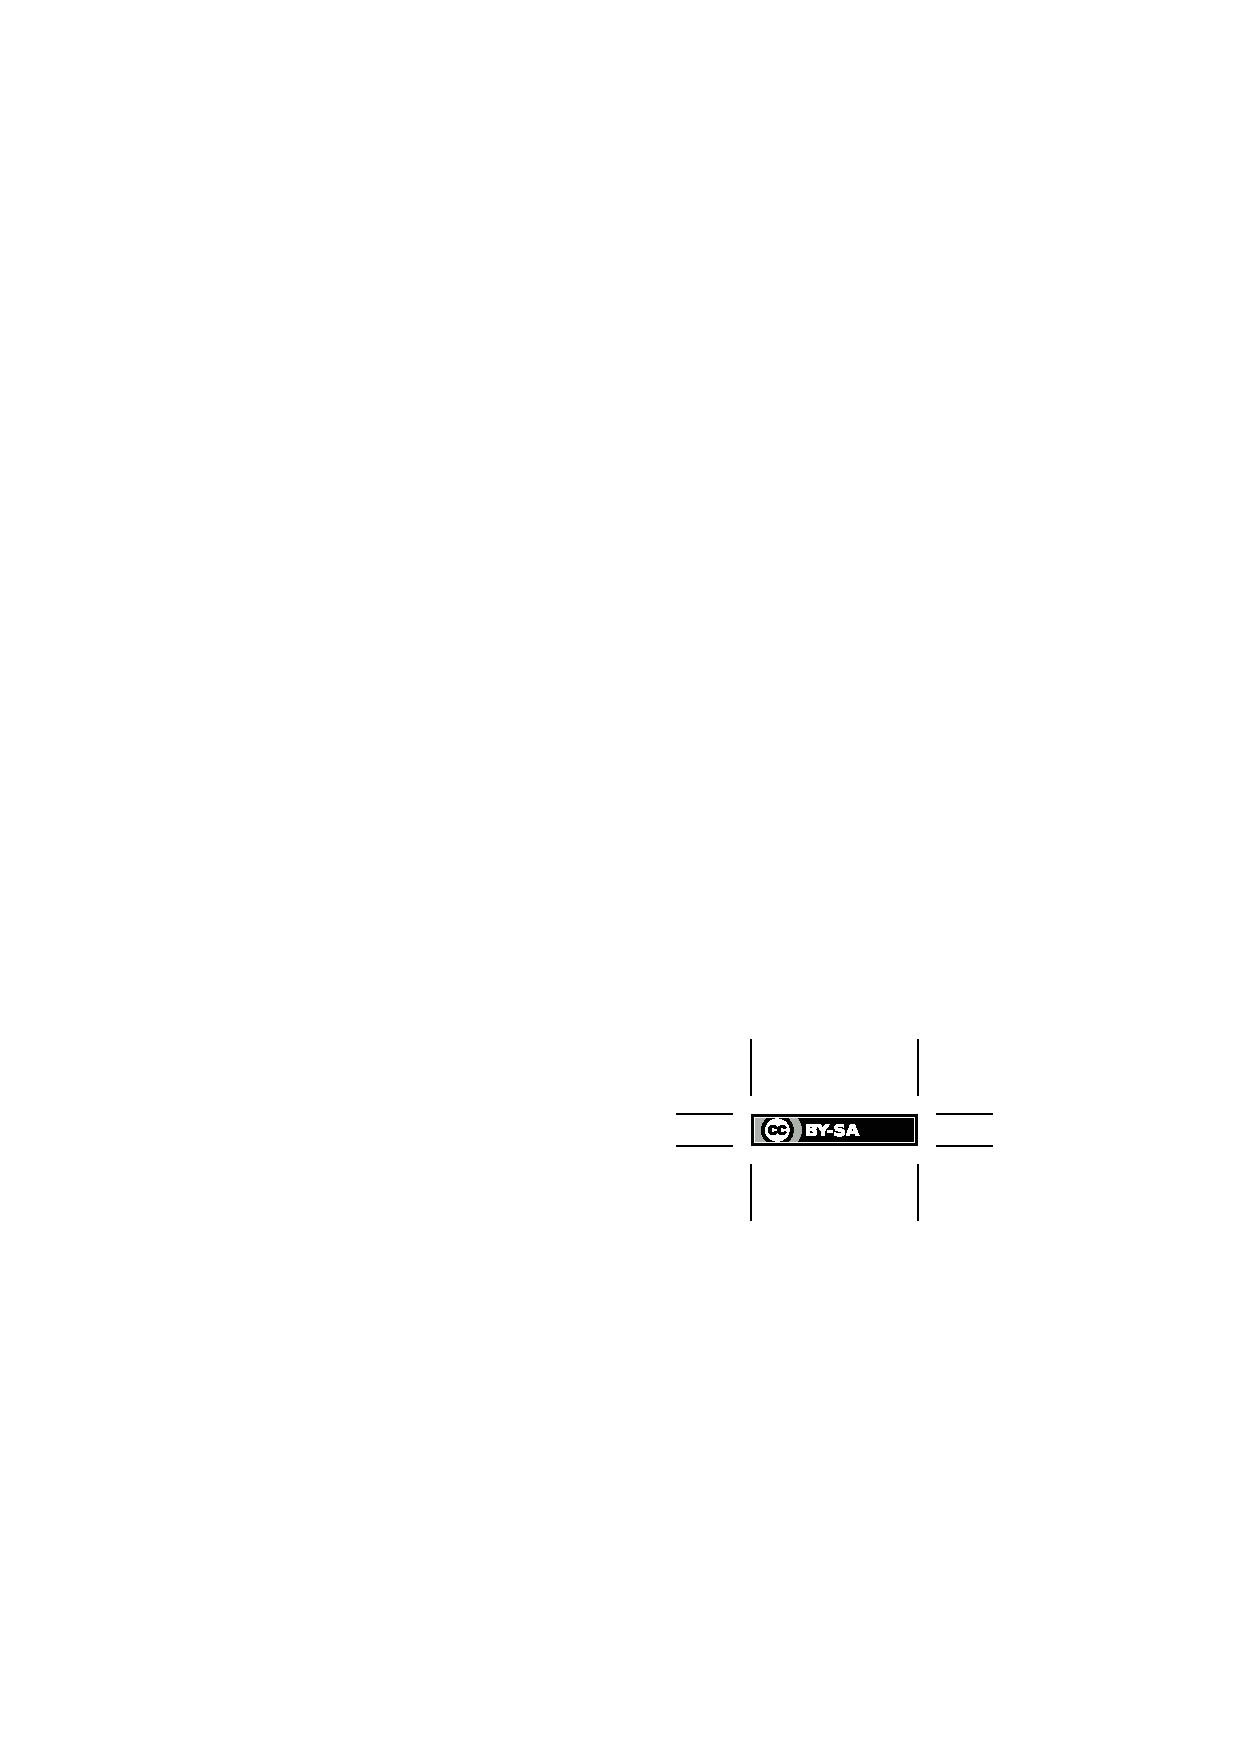
\includegraphics[height=1em]{fig/cc_by_sa_small}}}
%    \end{center}
%\end{frame}
%\note{
%}


\end{document}

